\section{Panorama energetico attuale}
La \textit{rete elettrica} attuale è il risultato di una rapida urbanizzazione e di un rapido sviluppo di infrastrutture in varie zone del mondo. Sebbene tali reti esistano ormai in molte aree geografiche diverse, le aziende generalmente tendono ad adottare tecnologie molto simili tra di loro. Ciononostante, restano altri fattori  legati allo sviluppo energetico di varia natura (economica, politica, geografica), che si diversificano a seconda dell'azienda. \newline
In generale però, pur tenendo in considerazione le differenze portate da tali fattori, la topologia base della rete elettrica attuale è rimasta immutata.
\begin{figure}[h] \centering{
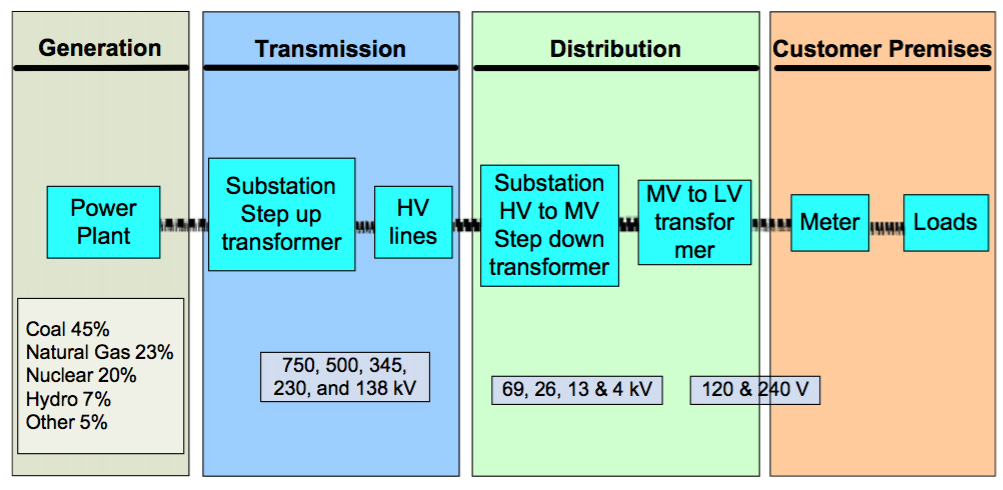
\includegraphics[scale=0.3, natwidth=1003,natheight=490]{imgs/elect_grid.png}}
\caption{La rete elettrica attuale}
\end{figure}
\newline La struttura della rete attuale è una struttura strettamente gerarchica. La figura 1.1 mostra l'esistenza di tre sottosistemi distinti: generazione, trasmissione e distribuzione. \newline Le centrali elettriche sono composte da generatori elettromeccanici i quali, spinti dal flusso dell'acqua corrente o da motori termici alimentati da combustioni chimiche, generano energia che, successivamente, viene inviata ai trasformatori del livello seguente, i quali la convertiranno in energia ad alto voltaggio per permettere trasmissioni a lunga distanza. Dopo tale step, si passa alla distribuzione, in cui si applica prima una trasformazione a medio voltaggio e, in seguito, si procede alla distribuzione agli utenti finali.
\newline Tale sistema è basato sostanzialmente su una comunicazione \textit{unidirezionale} in cui la sorgente non ha nessuna informazione real-time circa le necessità degli ultimi punti della catena. Pertanto si tende a sovraccaricare la rete, facendole raggiungere a priori i picchi massimi di carico; poiché è raro che le richieste degli utenti raggiungano tali valori, questo approccio porta a rendere la rete elettrica un meccanismo inefficiente.
\newline 
Inoltre, le reti elettriche attuali sono interconnesse tra loro a formare reti regionali o nazionali con lo scopo di fornire rotte ridondanti e alternative per il flusso della corrente in caso di problemi. \newline
La distribuzione dell'energia è gestita da un \textit{controllore centralizzato} che ha il compito di amministrare diverse regioni da un'unica posizione centrale. 
\section{Cenni storici}

\section{Perchè la Smart Grid}

\section{Cos'è una Smart Grid}

\section{Tecnologie coinvolte}